Dans la fenêtre \textit{Wiewertabs}, clicquer sur l'icône \textit{Edit amenagement}, sur la droite on dispose de la liste des aménagements existants.
Pour créer un nouvel aménagement, cliquer sur l'icône \textit{create new amenagement}, donner son nom (par exemple Champ) et sauvegarder.

\begin{figure}[!h]
	\begin{center}
	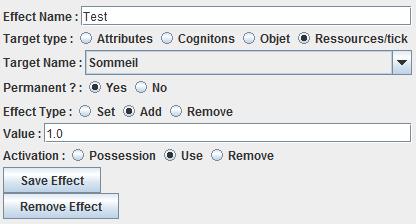
\includegraphics[scale=0.6]{DocumentationSimulation/images/effetsA.png}
	\caption[EFA]{Effet pour un aménagement \\}
	\label{EFA}
	\end{center}
	\end{figure}

 Tout comme pour les objets,  il est possible de saisir une recette pour la conception d'aménagements complexes, le processus étant identique à celui présenté dans la section sur les objets.
 De même, les aménagements peuvent avoir des effets ceux ci étant un peu différents de ceux présentés pour les objets (cf. Figure \ref{EFA})
 
 En effet,  les aménagements  ont la possibilité d'avoir pour cible (en sus des attributs ou caractéristiques d'agent et des cognitions)  des objets ou des ressources, et dans ce cas, l'effet ajoutera, modifiera ou bien supprimera l'objet sélectionné de l'inventaire, ou bien, modifiera, ajoutera, modifiera ou supprimera la ressource ciblée présente sur le patch où se situe l'aménagement.